\documentclass[11pt,a4paper]{article}

\usepackage[utf8]{inputenc}
\usepackage[T1]{fontenc}
\usepackage[english]{babel}
\usepackage[a4paper,margin=2.4cm]{geometry}

\usepackage{amsmath, amssymb, amsthm}
\usepackage{mathtools}
\usepackage{booktabs}
\usepackage{tabularx}
\usepackage{array}
\usepackage{caption}
\usepackage{float}
\usepackage{enumitem}
\usepackage{microtype}
\usepackage{xcolor}
\usepackage{listings}
\usepackage{fancyhdr}
\usepackage{titlesec}
\usepackage{tikz}
\usetikzlibrary{positioning, arrows.meta, fit, backgrounds, calc, shapes.geometric}
\usepackage{pgfplots}
\pgfplotsset{compat=1.18}
\usepackage[hidelinks]{hyperref}

%  ---  Sober palette: ink, two greys, one desaturated navy accent  ---
\definecolor{ink}{RGB}{26,30,36}
\definecolor{slate}{RGB}{92,101,112}
\definecolor{mist}{RGB}{233,235,238}
\definecolor{rulegrey}{RGB}{188,194,201}
\definecolor{steel}{RGB}{47,72,102}
\definecolor{steellight}{RGB}{124,146,172}

\hypersetup{
    colorlinks=true,
    linkcolor=steel,
    citecolor=steel,
    urlcolor=steel,
    pdftitle={Coordinating UGV Fleets under Epistemic Uncertainty},
    pdfauthor={Haniel Ulises},
}

\color{ink}

\pagestyle{fancy}
\fancyhf{}
\fancyhead[L]{\small\textcolor{slate}{\itshape Coordinating UGV Fleets under Epistemic Uncertainty}}
\fancyhead[R]{\small\textcolor{slate}{\thepage}}
\renewcommand{\headrulewidth}{0.4pt}
\renewcommand{\headrule}{\hbox to\headwidth{\color{rulegrey}\leaders\hrule height \headrulewidth\hfill}}

\titleformat{\section}{\normalfont\large\bfseries\color{ink}}{\thesection}{0.7em}{}
\titleformat{\subsection}{\normalfont\normalsize\bfseries\color{ink}}{\thesubsection}{0.7em}{}
\titleformat{\paragraph}[runin]{\normalfont\bfseries\color{slate}}{}{0em}{}[.]

\captionsetup{font=small, labelfont={bf,color=slate}, textfont=footnotesize}

\theoremstyle{definition}
\newtheorem{definition}{Definition}
\newtheorem{example}{Example}

\lstdefinestyle{epddl}{
    backgroundcolor=\color{mist},
    basicstyle=\ttfamily\scriptsize\color{ink},
    keywordstyle=\color{steel}\bfseries,
    commentstyle=\color{slate}\itshape,
    stringstyle=\color{slate},
    morecomment=[l]{;},
    morekeywords={define,domain,problem,requirements,predicates,types,action,event,
        parameters,precondition,effects,action-type,observability-conditions,goal,init,
        agents,objects,facts,facts-init,fact,forall,exists,imply,and,or,not,when,if,else,
        Fully,Partially,Oblivious,public-ontic,private-sensing,public-announcement,
        private-announcement},
    frame=single,
    rulecolor=\color{rulegrey},
    framesep=5pt,
    xleftmargin=6pt,
    xrightmargin=0pt,
    breaklines=true,
    showstringspaces=false,
    columns=fullflexible,
    captionpos=b,
}
\lstset{style=epddl}

%  ---  Notation  ---
\newcommand{\Ag}{\mathcal{A}}
\newcommand{\Prop}{\mathcal{P}}
\newcommand{\Kop}[1]{K_{#1}}
\newcommand{\Kw}[1]{\mathit{Kw}_{#1}}
\newcommand{\Cop}[1]{C_{#1}}
\newcommand{\Mod}{\mathcal{M}}
\newcommand{\Ev}{\mathcal{E}}
\newcommand{\prd}{\otimes}

\newcommand{\scenariohead}[1]{\vspace{2pt}\noindent\textcolor{steel}{\bfseries #1}\par\vspace{1pt}}

\begin{document}

\begin{titlepage}
\centering
\vspace*{2.4cm}
{\color{rulegrey}\rule{\textwidth}{0.8pt}}\\[0.9cm]
{\LARGE\bfseries Coordinating UGV Fleets under\\[0.25cm] Epistemic Uncertainty\par}
\vspace{0.5cm}
{\large\color{slate} A Dynamic-Epistemic-Logic Formulation of the Planning Problem,\\ with a Scaling Benchmark\par}
\vspace{0.7cm}
{\color{rulegrey}\rule{\textwidth}{0.8pt}}\\[1.4cm]

{\large Haniel Ulises\par}
\vspace{0.3cm}
{\color{slate} Epistemic Robotics}\\
\vspace{0.15cm}
{\color{slate}\today}

\vfill
\begin{minipage}{0.86\textwidth}
\small\color{slate}
\textbf{Abstract.}\ Fleets of unmanned ground vehicles that sense locally and
communicate imperfectly face a coordination problem that is not captured by
classical planning over world states: what has to be achieved is a
configuration of \emph{knowledge} across the fleet, and the actions that
achieve it, sensing, driving into radio range, relaying a report, are
valuable only for their epistemic effect. This report formulates that problem
in Dynamic Epistemic Logic (DEL), where an epistemic state is a Kripke model
and an action is an event model applied by product update, and it states the
resulting planning problem: from a multi-pointed initial model, find a policy
whose branches are the designated events of sensing actions and whose leaves
all satisfy a modal goal formula. Six coordination scenarios, facility-wide
broadcast, range-limited radio, second-order goals, deployment geometry,
addressed radio with selective-disclosure goals, and a heterogeneous fleet
whose capabilities interlock, are described conceptually and encoded as four
EPDDL domains. A benchmark of 204 instances, scaling the fleet size, the
facility size, the amount of initial uncertainty, and the number of items to
localise, is grounded with the \textsf{plank} toolkit and solved with the
\textsf{aletheia} planner; 196 are solved under a 60\,s budget.
The measurements separate two costs that are easily conflated: grounding
scales with fleet size times facility size, while search is dominated by the
number of worlds the fleet initially considers possible, three orders of
magnitude across the grid, against one for fleet size. Restricted
communication costs a further factor of three and accounts for every unsolved
instance. The suite also isolates a reproducible correctness fault in the
planner, on goals conjoining knowledge requirements over several atoms.
\end{minipage}
\vspace{1.2cm}
\end{titlepage}

\tableofcontents
\thispagestyle{empty}
\clearpage
\setcounter{page}{1}

%======================================================================
\section{Introduction}

A team of unmanned ground vehicles (UGVs) inspecting a facility rarely fails
because its members cannot compute a route. It fails because one vehicle knows
something the others do not, and no one has established who knows what. A
vehicle that has scanned a bay and found the target holds information that is
useless until it is transmitted; a vehicle that transmits out of radio range
has changed nothing; a vehicle that must act only once it is sure a teammate
has received a report needs to reason about the teammate's knowledge, not just
about the world.

Classical planning has no vocabulary for this. Its state is an assignment to
propositions, and its goal is a condition on that assignment. It can express
\emph{the target is in bay 4}; it cannot express \emph{every vehicle knows
which bay the target is in}, still less \emph{$R_1$ knows that $R_2$ knows}.
Contingent and conformant planning add uncertainty but keep the perspective
single-agent: they model what \emph{the planner} does not know, not what the
individual vehicles know about each other.

Dynamic Epistemic Logic (DEL) supplies exactly the missing vocabulary. A state
of affairs is a Kripke model whose worlds are the situations the agents
consider possible and whose accessibility relations encode, per agent, which
situations that agent cannot tell apart. An action is a second Kripke-style
structure, an event model, whose events carry preconditions and
postconditions and whose relations encode who observes what. Executing an
action is the product update of the two structures. Because observation is
part of the action's definition, the same physical act can be public, private,
or unobserved depending only on the observability relation attached to it, and
that distinction is precisely the one that governs UGV coordination.

This report has three purposes, and deliberately stops short of a fourth. It
(i) states the UGV coordination problem as a DEL planning problem; (ii)
describes, conceptually, four scenario families in which the epistemic
structure of the problem changes qualitatively; and (iii) reports a scaling
benchmark that measures where a current DEL planner stops being practical on
them. It does \emph{not} address execution, ROS~2 integration, controller
synthesis, or perception; those concerns are orthogonal to the planning
problem treated here and are the subject of a companion document.

%======================================================================
\section{Background: the planning problem}

\subsection{Epistemic language}

Fix a finite set $\Ag$ of agents (the vehicles) and a finite set $\Prop$ of
atomic propositions. The language $\mathcal{L}$ is

\[
\varphi ::= p \mid \neg\varphi \mid \varphi\wedge\varphi \mid \Kop{i}\varphi
      \mid \Cop{G}\varphi , \qquad p\in\Prop,\; i\in\Ag,\; G\subseteq\Ag .
\]

$\Kop{i}\varphi$ reads \emph{agent $i$ knows $\varphi$} and $\Cop{G}\varphi$
\emph{$\varphi$ is common knowledge in $G$}. Two derived operators carry most
of the weight in what follows:

\[
\Kw{i}\varphi \;\equiv\; \Kop{i}\varphi \vee \Kop{i}\neg\varphi ,
\qquad\qquad
\widehat{\Kw{i}}\varphi \;\equiv\; \neg\Kw{i}\varphi .
\]

$\Kw{i}\varphi$, \emph{$i$ knows whether $\varphi$}, is the natural form
of an information-gathering goal: the fleet is not asked to make the target be
in a particular bay, only to find out which bay it is in. Its dual states
ignorance, and is how an initial state says that nobody knows yet.

\subsection{Epistemic states and actions}

\begin{definition}[Epistemic state]
An epistemic state is a multi-pointed Kripke model
$\Mod = (W, \{R_i\}_{i\in\Ag}, V, W_d)$ where $W$ is a finite set of worlds,
$R_i\subseteq W\times W$ is agent $i$'s indistinguishability relation, $V:W\to
2^{\Prop}$ is a valuation, and $\emptyset\neq W_d\subseteq W$ is the set of
\emph{designated} worlds, those that are candidates for the actual one.
Knowledge is modelled in $\mathrm{S5}$: each $R_i$ is an equivalence relation.
\end{definition}

The size of $W_d$ is the modeller's statement about what is objectively open.
If the true bay of the target is asserted in the initial state, $|W_d| = 1$ and
the planner may exploit knowledge the vehicles do not have; leaving it open
gives $|W_d| > 1$ and forces a plan that works for every candidate. This
distinction is not cosmetic, Section~\ref{sec:bench} keeps every benchmark
instance in the open setting for exactly this reason.

\begin{definition}[Event model]
An action is an event model $\Ev = (E, \{Q_i\}_{i\in\Ag}, \mathit{pre},
\mathit{post}, E_d)$: $E$ is a finite set of events, $Q_i\subseteq E\times E$
says which events agent $i$ cannot distinguish, $\mathit{pre}: E\to\mathcal{L}$
gives each event an epistemic precondition, $\mathit{post}$ assigns literal
postconditions, and $E_d\subseteq E$ are the designated events, the outcomes
that may actually occur.
\end{definition}

\begin{definition}[Product update]
$\Mod\prd\Ev$ has worlds $\{(w,e) : \Mod,w\models \mathit{pre}(e)\}$, relation
$(w,e)\mathrel{R'_i}(v,f)$ iff $w\mathrel{R_i}v$ and $e\mathrel{Q_i}f$,
valuation revised by $\mathit{post}(e)$, and designated worlds
$\{(w,e) : w\in W_d,\, e\in E_d\}$.
\end{definition}

The observability relation $Q_i$ is the whole modelling story. An event model
whose events are all $Q_i$-distinguishable for every $i$ is a public action; if
some agent relates every event to a distinguished \emph{null} event, that agent
is \emph{oblivious}, unaware not only of the outcome but of the occurrence.
Obliviousness is the feature that makes short-range radio interesting: a
vehicle out of range does not know that a report was sent, so it cannot even
infer that its teammates are now better informed.

\subsection{The planning task}

\begin{definition}[Epistemic planning task]
A task is $\Pi = (\Mod_0, \mathcal{A}, \gamma)$ with $\Mod_0$ an initial
epistemic state, $\mathcal{A}$ a finite set of ground actions (event models),
and $\gamma\in\mathcal{L}$ a goal formula. An action $a$ is applicable in
$\Mod$ when every designated world of $\Mod$ satisfies $\mathit{pre}$ of some
designated event of $a$.
\end{definition}

A sensing action has more than one designated event, one per possible
reading, and the executing agent learns which one occurred. A solution is
therefore not a sequence but a \emph{policy}, naturally represented as an
AND/OR tree: OR-nodes choose an action, AND-nodes branch over the designated
events of that action, and every leaf must satisfy $\gamma$. When no action in
a plan has more than one designated event, the tree degenerates to a sequence
and the task is a sequential epistemic planning problem.

Two properties of this problem shape everything downstream. First, plan
existence is undecidable in general: unrestricted event models with epistemic
preconditions can encode arbitrary computation, and decidability is recovered
only under restrictions such as bounding modal depth or forbidding
postconditions. Second, even in the decidable fragments the state
representation grows multiplicatively, $|W|$ after $k$ product updates is
bounded by $|W_0|\cdot\prod_{j\le k}|E_j|$, so the practical limit is set by
how quickly the model grows along the search frontier, not by the length of the
plan.

\subsection{From specification to search: the toolchain}

The scenarios below are written in EPDDL, a PDDL-style specification language
for DEL tasks in which one declares events with epistemic preconditions,
reusable \emph{action types} (public/private/semi-private ontic, sensing, and
announcement templates), and per-agent observability conditions that may
themselves be formulas. The \textsf{plank} toolkit parses, type-checks, and
grounds a specification into an explicit JSON task; the \textsf{aletheia}
planner reads that task and searches. Figure~\ref{fig:pipeline} shows the
pipeline used throughout.

\begin{figure}[H]
\centering
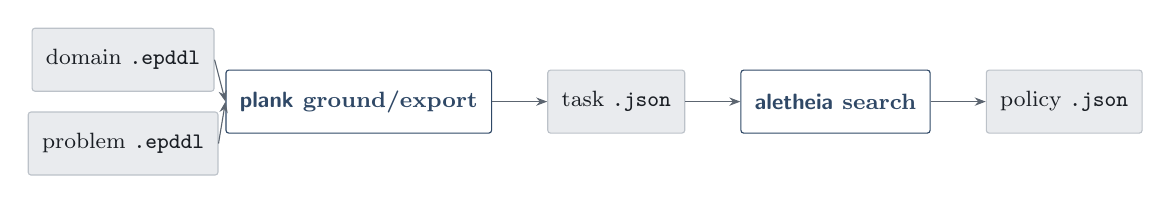
\begin{tikzpicture}[
    box/.style={draw=rulegrey, fill=mist, rounded corners=1pt, minimum height=8mm,
                inner xsep=5pt, font=\footnotesize, text=ink},
    dark/.style={box, draw=steel, fill=white, text=steel, font=\footnotesize\bfseries},
    arr/.style={-{Stealth[length=4pt]}, draw=slate}
  ]
  \node[box] (dom) {domain \texttt{.epddl}};
  \node[box, below=2.5mm of dom] (prob) {problem \texttt{.epddl}};
  \node[dark, right=13mm of $(dom)!0.5!(prob)$] (plank) {\textsf{plank} ground/export};
  \node[box, right=7mm of plank] (json) {task \texttt{.json}};
  \node[dark, right=7mm of json] (alet) {\textsf{aletheia} search};
  \node[box, right=7mm of alet] (plan) {policy \texttt{.json}};
  \draw[arr] (dom.east) -- (plank.west);
  \draw[arr] (prob.east) -- (plank.west);
  \draw[arr] (plank) -- (json);
  \draw[arr] (json) -- (alet);
  \draw[arr] (alet) -- (plan);
\end{tikzpicture}
\caption{Specification-to-policy pipeline. Grounding is where the fleet size
and corridor length turn into ground actions; search is where the epistemic
model grows.}
\label{fig:pipeline}
\end{figure}

%======================================================================
\section{From robot software to epistemic models}
\label{sec:abstraction}

The formalism of Section~2 talks about worlds and accessibility relations; a
UGV stack talks about occupancy grids, pose estimates, sensor footprints and
link budgets. This section states the correspondence, because the epistemic
planning problem is only well posed once it is fixed.

\subsection{Metric map to symbolic state}

The navigation layer maintains a metric occupancy grid: a discretisation of the
facility into cells, each free, occupied, or unknown. Planning over that grid
directly is hopeless for an epistemic planner, a $20\times 6$ grid already
gives $2^{120}$ valuations before any modality is added. The standard remedy is
the standard one in task-and-motion architectures: quotient the free space into
a small set of \emph{regions} whose adjacency graph is what the task layer
reasons about. Here the regions are bays, obtained from the shelving structure,
and the adjacency relation \texttt{(adjacent b$_i$ b$_j$)} is a static fact of
the EPDDL problem. Figure~\ref{fig:abstraction} shows the quotient.

\begin{figure}[H]
\centering
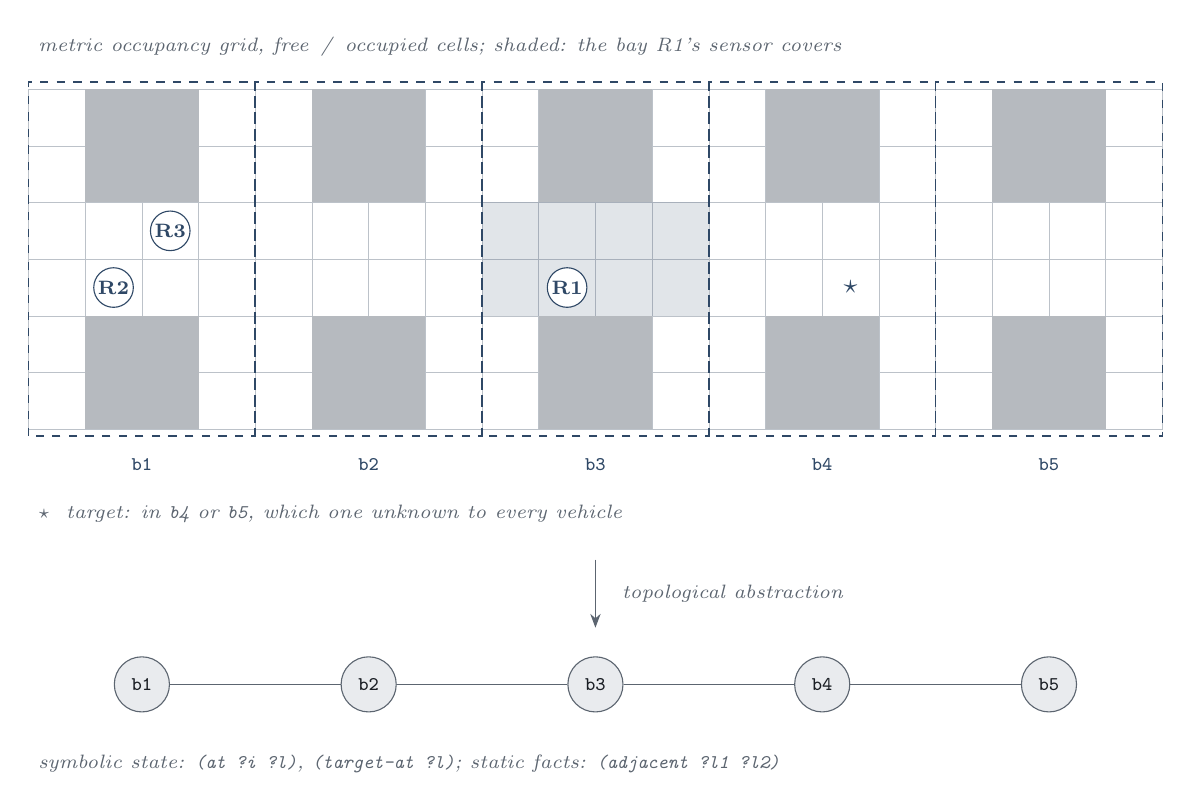
\begin{tikzpicture}[x=7.2mm, y=7.2mm,
    ugv/.style={circle, draw=steel, fill=white, text=steel, font=\bfseries\scriptsize,
                inner sep=0.8pt, minimum size=4.6mm},
    note/.style={font=\scriptsize\itshape, text=slate}
  ]
  % --- occupancy grid ---
  \foreach \x in {0,...,19} \foreach \y in {0,...,5} {
      \draw[draw=rulegrey, line width=0.2pt, fill=white] (\x,\y) rectangle ++(1,1);
  }
  % shelving blocks (occupied cells)
  \foreach \bx in {0,4,8,12,16} {
    \foreach \dx in {1,2} \foreach \y in {0,4} {
        \fill[slate!45] (\bx+\dx,\y) rectangle ++(1,2);
    }
  }
  % sensor footprint of the bay R1 occupies
  \fill[steel, opacity=0.14] (8,2) rectangle ++(4,2);

  % UGVs in the corridor band
  \node[ugv] at (1.5,2.5) {R2};
  \node[ugv] at (2.5,3.5) {R3};
  \node[ugv] at (9.5,2.5) {R1};
  \node[text=steel, font=\normalsize] at (14.5,2.5) {$\star$};

  % bay partition
  \foreach \bx/\lab in {0/b1, 4/b2, 8/b3, 12/b4, 16/b5} {
      \draw[draw=steel, dashed, line width=0.6pt] (\bx,-0.12) rectangle (\bx+4,6.12);
      \node[font=\scriptsize\ttfamily, text=steel] at (\bx+2,-0.62) {\lab};
  }
  \node[note, anchor=west] at (0,6.75)
       {metric occupancy grid, free \,/\, occupied cells; shaded: the bay R1's sensor covers};
  \node[note, anchor=west] at (0,-1.5)
       {$\star$\ \ target: in \texttt{b4} or \texttt{b5}, which one unknown to every vehicle};

  % --- arrow ---
  \draw[-{Stealth[length=5pt]}, draw=slate] (10,-2.3) -- (10,-3.5);
  \node[note, anchor=west] at (10.3,-2.9) {topological abstraction};

  % --- symbolic graph ---
  \foreach \i/\x/\lab in {1/2/b1, 2/6/b2, 3/10/b3, 4/14/b4, 5/18/b5} {
      \node[circle, draw=slate, fill=mist, minimum size=7mm,
            font=\scriptsize\ttfamily, text=ink, inner sep=0.5pt] (n\i) at (\x,-4.5) {\lab};
  }
  \foreach \i in {1,...,4} {
      \pgfmathtruncatemacro{\j}{\i+1}
      \draw[draw=slate] (n\i) -- (n\j);
  }
  \node[note, anchor=west] at (0,-5.9)
       {symbolic state: \texttt{(at ?i ?l)}, \texttt{(target-at ?l)};
        static facts: \texttt{(adjacent ?l1 ?l2)}};
\end{tikzpicture}
\caption{The abstraction the task layer plans over. Cells are quotiented into
bays; the sensor footprint is assumed to cover exactly the occupied bay, which
is what licenses \texttt{scan} being a bay-local sensing action; the adjacency
graph of bays becomes static facts in the EPDDL problem.}
\label{fig:abstraction}
\end{figure}

Three modelling commitments are hidden in that picture, and each is an
assumption the robotics layer must actually discharge.

\begin{enumerate}[leftmargin=1.4em, itemsep=2pt]
\item \textbf{Navigation is assumed to succeed.} \texttt{move} is a
deterministic ontic action with public observability. That is only sound if the
navigation stack reaches the commanded bay, and if fleet pose is shared, a
position feed the vehicles all subscribe to. If either fails, movement itself
becomes an epistemic action with uncertain outcome, which multiplies the model
in exactly the way Section~\ref{sec:results} shows is expensive.
\item \textbf{The sensor is bay-local and reliable.} \texttt{scan} has one
designated event per reading and no false positives. A real detector with a
miss rate would need either a probabilistic treatment, which DEL in this form
does not provide, or a conservative encoding in which a negative reading does
not license the inference the planner exploits.
\item \textbf{Connectivity is a function of position.} The range predicate , 
same bay or adjacent bay, stands in for a link budget. This is the
assumption that most deserves scrutiny in a real facility, and also the one
that is cheapest to change: it is a single observability condition in the
domain.
\end{enumerate}

\subsection{Where the epistemic layer sits}

The planner produces a policy, not a trajectory. Its actions are commands to
the layer beneath, \emph{drive to bay $b_3$}, \emph{run the detector},
\emph{transmit this report}, and its branches are conditioned on sensing
outcomes the layer beneath reports back. In an autonomy stack, this is a
deliberative layer above navigation and below mission specification, and its
distinguishing feature is that its state is not the fleet's position but the
fleet's \emph{information}. Execution is then the usual loop: dispatch the
action at the current policy node, wait for the outcome, descend the
corresponding branch, and replan if an outcome falls outside the model. This
report treats only the synthesis of that policy; the execution and interface
questions are the subject of the companion document.

%======================================================================
\section{Coordination scenarios}
\label{sec:scenarios}

All four scenarios share one physical setting, deliberately austere so that
the epistemic structure is not confounded with geometric difficulty. A
facility is a corridor of $L$ bays $b_1,\dots,b_L$, adjacent in sequence. A
fleet of $N$ UGVs drives between adjacent bays. A target sits in exactly one of
the last $U$ bays; which one is not known to anybody. Each vehicle carries a
sensor that reads only the bay it occupies, and a radio.

\begin{figure}[H]
\centering
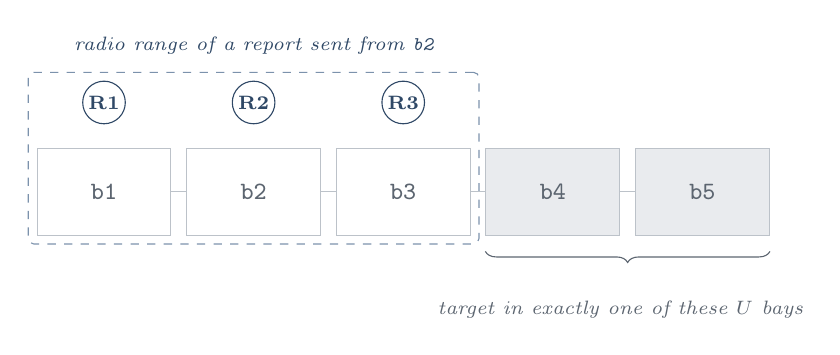
\begin{tikzpicture}[
    bay/.style={draw=rulegrey, fill=white, minimum width=17mm, minimum height=11mm,
                font=\small\ttfamily, text=slate},
    cand/.style={bay, fill=mist},
    ugv/.style={draw=steel, fill=white, text=steel, circle, inner sep=1.2pt,
                font=\scriptsize\bfseries},
    lbl/.style={font=\scriptsize\itshape, text=slate}
  ]
  \foreach \i in {1,...,3} { \node[bay] (b\i) at (\i*19mm, 0) {b\i}; }
  \foreach \i in {4,5} { \node[cand] (b\i) at (\i*19mm, 0) {b\i}; }
  \foreach \i in {1,...,4} {
     \draw[draw=rulegrey] (b\i.east) -- (b\the\numexpr\i+1\relax.west); }

  \node[ugv, above=3mm of b1] (r1) {R1};
  \node[ugv, above=3mm of b2] (r2) {R2};
  \node[ugv, above=3mm of b3] (r3) {R3};

  \draw[decorate, decoration={brace, mirror, amplitude=4pt}, draw=slate]
        ($(b4.south west)+(0,-2mm)$) -- ($(b5.south east)+(0,-2mm)$);
  \node[lbl, below=7mm of $(b4.south east)$] {target in exactly one of these $U$ bays};

  \begin{scope}[on background layer]
    \node[draw=steellight, dashed, rounded corners=2pt, fit=(b1)(b3)(r1)(r3),
          inner sep=3pt] (range) {};
  \end{scope}
  \node[lbl, above=1mm of range.north, text=steel] {radio range of a report sent from \texttt{b2}};
\end{tikzpicture}
\caption{The shared setting: a corridor of $L$ bays, $N$ UGVs, target
uncertainty confined to the last $U$ bays, and, in the range-limited
scenarios, a radio that reaches only the sender's bay and its neighbours.}
\label{fig:setting}
\end{figure}

Two epistemic actions are available to every vehicle. \textbf{Scan} is private
sensing: vehicle $i$ standing in bay $l$ learns whether the target is there,
and the rest of the fleet observes nothing, not the reading, not the scan.
\textbf{Report} is an announcement whose precondition is epistemic,
$\Kop{i}\,\mathit{target\text{-}at}(l)$: a vehicle can only report what it
actually knows. What changes across scenarios is who hears it.

\scenariohead{S1, Facility-wide radio.}
The report is a public announcement: every vehicle receives it, and because
reception is itself public, the content becomes common knowledge in one step.
The planning problem is a division of labour: which vehicle drives to which
candidate bay, in what order, and when does it speak. The epistemic subtlety
is already present in the negative branch. A vehicle that scans $b_4$ and finds
nothing has learned, given the common knowledge that the target is in exactly
one of $\{b_4,b_5\}$, that it is in $b_5$, and can report \emph{that} even
though it never observed $b_5$. A planner that does not reason about the agent's
knowledge, only about observations, cannot find this two-step solution and will
send a vehicle down the corridor to confirm what is already entailed.

\scenariohead{S2, Range-limited radio.}
The report reaches only vehicles in the sender's bay or an adjacent one;
everyone else is oblivious to it. Sensing and communicating now pull the fleet
in opposite directions: information is acquired at the far end of the corridor
and must be delivered where the fleet is. Three qualitatively different
solutions exist, and which is cheapest is an instance property, not a domain
property: the scanning vehicle drives back into range and reports; a second
vehicle positions itself as a relay so that a chain of in-range reports
propagates the finding; or the fleet agrees to rendezvous. Obliviousness is
what makes this hard to approximate. A vehicle out of range does not merely
miss the content, it does not learn that a report happened, so no amount of
subsequent inference recovers the information without a further transmission.

\scenariohead{S3, Second-order goals.}
The goal is not fleet-wide knowledge but $\Kop{R_1}\Kw{R_2}\,\mathit{target
\text{-}at}(b)$: $R_1$ must know that $R_2$ knows where the target is. This is
the planning form of delegation, $R_1$ may only stand down, or move on to
another task, once it is sure its teammate has what it needs. Under a public
radio the goal is nearly free, since public announcement produces common
knowledge and common knowledge entails every finite nesting. Under a
range-limited radio it is the genuinely hard case: $R_1$ must establish that
its report was \emph{received}, which requires reasoning about $R_2$'s
observability condition, that is, about whether $R_2$ was in an adjacent bay
at transmission time. Goals of this shape are where DEL earns its cost;
nothing weaker expresses them.

\scenariohead{S4, Deployment geometry.}
The two deployments, all vehicles starting at a depot ($b_1$) versus spread
round-robin along the corridor, change no formula, only the initial model.
Yet they change the character of the solution. From a depot, the fleet must
first travel, and the plan is dominated by ontic movement whose only purpose is
to enable a later sensing action; the epistemic content is concentrated at the
end. Spread out, some vehicle is typically already near a candidate bay, so
sensing starts immediately, but under range-limited radio the fleet is now
dispersed beyond mutual reach and the delivery problem of S2 is worse. This
scenario is included because it isolates a fact that is easy to miss when
reading plans: in epistemic planning, the initial \emph{geometry} determines
how much of the search is spent on non-epistemic actions.

\subsection{Extended settings}

The four families above vary the observability model over a fixed physical
setting. Two further families vary the setting itself, and each reaches
something the corridor families cannot express.

\scenariohead{S5, Addressed radio and selective disclosure.}
Communication is point-to-point: \texttt{tell} is received by exactly the
addressee, and every other vehicle is oblivious to it. Only one UGV in the
fleet carries a detector, so knowledge must travel by radio rather than each
vehicle driving out to look. This model reaches information states a broadcast
cannot: under S1 every transmission produces common knowledge, so the fleet's
knowledge is always symmetric, whereas here one teammate can be informed while
another is deliberately left ignorant. The corresponding goal is
\emph{selective}: $\Kw{R_2}\,p \wedge \neg\Kw{R_3}\,p$. Goals of that shape , 
a negated modality, are the reason the epistemic state has to be represented
rather than summarised: no measure of ``how much the fleet knows'' can express
that one particular vehicle must \emph{not} know something.

\scenariohead{S6, Interlocking capabilities.}
The fleet is heterogeneous and the facility is not fully traversable. One
vehicle carries the detector, another carries the key, and a bay in the middle
of the corridor starts locked, so neither vehicle can complete the mission
alone: the keyholder must open the way before the scanner-equipped vehicle can
reach the far bays, and the reading must then be broadcast. Several items must
be localised, which multiplies the initial model, two independent binary
uncertainties give four worlds rather than two. This family is where ontic
cooperation and epistemic cooperation interleave: the plans alternate between
actions taken to change the world so that information can be acquired, and
actions taken to distribute information already held.

\smallskip
Table~\ref{tab:scenarios} summarises the six families and what each one asks
of the planner.

\begin{table}[H]
\centering
\small
\caption{The scenario families, their goal formulas, and the reasoning each
requires. S1--S4 share the corridor setting and vary only observability;
S5--S6 vary the setting itself.}
\label{tab:scenarios}
\begin{tabularx}{\textwidth}{@{}l l >{\raggedright\arraybackslash}X@{}}
\toprule
\textbf{Family} & \textbf{Goal} & \textbf{What the planner must discover} \\
\midrule
S1 Public radio & $\Cop{\Ag}\bigwedge_{i}\Kw{i}\,p_b$ &
Division of labour; inferring the target bay from a negative scan. \\
S2 Range-limited & $\Cop{\Ag}\bigwedge_{i}\Kw{i}\,p_b$ &
Return, relay, or rendezvous to deliver knowledge past obliviousness. \\
S3 Second-order & $\Kop{R_1}\Kw{R_2}\,p_b$ &
Establishing that a report was received, from $R_2$'s observability condition. \\
S4 Geometry & either & How much ontic travel must precede any epistemic gain. \\
\addlinespace
S5 Addressed radio & $\Kw{R_2}\,p_b \wedge \neg\Kw{R_3}\,p_b$ &
Whom to tell, once the fleet's knowledge is allowed to be asymmetric. \\
S6 Facility & $\Cop{\Ag}\bigwedge_{i,o}\Kw{i}\,p_{o,b}$ &
Interleaving ontic cooperation (unlock) with epistemic cooperation (scan, report). \\
\bottomrule
\end{tabularx}
\end{table}

%======================================================================
\section{Benchmark design}
\label{sec:bench}

\subsection{Domains}

The scenarios are encoded as two EPDDL domains sharing predicates and the
\texttt{move}/\texttt{scan} actions and differing only in the announcement.
\texttt{ugv-public} gives \texttt{broadcast} the \emph{public-announcement}
action type with \texttt{(default Fully)}; \texttt{ugv-radio} gives
\texttt{report} the \emph{private-announcement} type with a per-agent
observability condition that evaluates the range predicate. The listing below
is that condition, the one place where the two domains part company.

\begin{lstlisting}[caption={Range-limited radio: observability as a formula. A
vehicle hears the report iff it shares a bay with the sender or occupies an
adjacent one; otherwise it is oblivious to the transmission.}, captionpos=b]
(:action report
    :parameters (?i - agent ?l - location)
    :action-type (private-announcement (e-report ?i ?l) (nil))
    :observability-conditions
        (:and
            (?i Fully)
            (:forall (?j - agent | (/= ?i ?j))
                (?j
                    (if
                        (forall (?l1 - location)
                            (imply
                                (at ?i ?l1)
                                (exists (?l2 - location |
                                        (or (= ?l2 ?l1) (adjacent ?l1 ?l2) (adjacent ?l2 ?l1)))
                                    (at ?j ?l2) )))
                        Fully
                    else
                        Oblivious ) ) )
            (default Oblivious) )
)
\end{lstlisting}

Note that \texttt{scan} is deliberately \emph{private} sensing in both domains:
without it, a fleet would learn everything by watching each other and no
communication would ever be necessary. The interplay between private
acquisition and restricted communication is the whole problem.

\subsection{Instance family}

Instances cross five parameters: domain (\texttt{public}, \texttt{radio}),
fleet size $N\in\{2,3,4\}$, corridor length $L\in\{3,4,5,6\}$, uncertainty
$U\in\{2,3,4\}$ candidate bays, deployment (\texttt{depot}, \texttt{spread}),
and goal (\texttt{ck}, \texttt{nested}). Combinations with $U > L-1$ are
excluded, and the far corner of the grid is kept sparse, giving
\textbf{144 instances}. Every instance leaves the true bay unasserted, so all
$U$ candidate worlds remain designated and no plan may exploit information the
fleet does not have.

Instances are generated by \texttt{gen\_instances.py} and swept by
\texttt{run\_benchmark.py}, which grounds each with \textsf{plank}, solves it
with \textsf{aletheia} under a 60~s limit, and records the task size, the
selected heuristic and strategy, the search effort, and wall-clock times.

\begin{table}[H]
\centering
\small
\caption{The instance family. Ground-action counts are the range over the
instances of each family after grounding with \textsf{plank}.}
\label{tab:family}
\begin{tabular}{@{}l r r r r@{}}
\toprule
\textbf{Family} & \textbf{Instances} & \textbf{Depot} & \textbf{Spread} & \textbf{Ground actions} \\
\midrule
S1 public / CK & 36 & 18 & 18 & 20--88 \\
S2 radio / CK & 36 & 18 & 18 & 20--72 \\
S3a public / nested & 36 & 18 & 18 & 20--88 \\
S3b radio / nested & 36 & 18 & 18 & 20--72 \\
\midrule
Total & 144 & 72 & 72 & \\
\bottomrule
\end{tabular}
\end{table}


\subsection{Extended instances}

A further \textbf{60 instances} (\texttt{gen\_instances\_x.py}) cover S5 and
S6, bringing the suite to \textbf{204}. The addressed-radio family crosses
$N\in\{2,3,4\}$, $L\in\{3,4,5\}$, $U\in\{2,3\}$ and both deployments with the
second-order and selective goals, the latter only for $N\ge3$ since it needs a
third vehicle to keep ignorant. The facility family crosses $N\in\{2,3\}$ with
$(L,I)\in\{(4,1),(4,2),(5,1),(5,2),(6,1)\}$ items, each item confined to two
candidate bays, so $|W| = 2^{I}$.

Two structural differences from the corridor grid are worth stating, because
they show up in the measurements. Addressed communication is quadratic in the
fleet, \texttt{tell} grounds to $N(N{-}1)L$ actions against $NL$ for a
broadcast, so the extended family reaches larger action sets at smaller
fleet sizes. And the facility family is the only one in which the fleet must
change the world before it can learn anything: the locked bay makes an ontic
action a precondition for a sensing action, which lengthens every policy.

%======================================================================
\section{Results}
\label{sec:results}

\begin{table}[H]
\centering
\small
\caption{Coverage and cost by scenario family, under a 60\,s search budget.
Depth is the depth of the policy tree, leaves its number of terminal branches;
both are medians over solved instances, as are the times.}
\label{tab:coverage}
\begin{tabular}{@{}l r r r r r r r@{}}
\toprule
\textbf{Family} & \textbf{Solved} & \textbf{Cov.} & \textbf{Depth} & \textbf{Leaves}
 & \textbf{Expanded} & \textbf{Search (s)} & \textbf{Ground (s)} \\
\midrule
S1 public / CK & 36/36 & 100\% & 4 & 2 & 1397 & 0.01 & 0.08 \\
S2 radio / CK & 32/36 & 89\% & 5 & 2 & 4829 & 0.04 & 0.09 \\
S3a public / nested & 36/36 & 100\% & 4 & 2 & 1397 & 0.01 & 0.08 \\
S3b radio / nested & 32/36 & 89\% & 5 & 2 & 4164 & 0.03 & 0.10 \\
\midrule
All & 136/144 & 94\% & 5 & 2 & 2263 & 0.02 & 0.09 \\
\bottomrule
\end{tabular}
\end{table}


\begin{table}[H]
\centering
\small
\caption{Scaling along each parameter, aggregated over all other parameters.
Worlds is $|W|$ of the grounded initial model; expanded nodes and search time
are medians over the solved instances in each stratum.}
\label{tab:scaling}
\begin{tabular}{@{}l r r r r r@{}}
\toprule
\textbf{Stratum} & \textbf{Solved} & \textbf{Ground actions} & \textbf{Worlds}
 & \textbf{Expanded} & \textbf{Search (s)} \\
\midrule
Fleet $N$ $= 2$ & 48/48 & 32 & 2 & 1026 & 0.01 \\
Fleet $N$ $= 3$ & 44/48 & 42 & 2 & 3358 & 0.03 \\
Fleet $N$ $= 4$ & 44/48 & 56 & 2 & 6970 & 0.06 \\
\addlinespace
Corridor $L$ $= 3$ & 24/24 & 30 & 2 & 66 & 0.00 \\
Corridor $L$ $= 4$ & 48/48 & 42 & 2 & 1026 & 0.01 \\
Corridor $L$ $= 5$ & 48/48 & 54 & 2 & 6654 & 0.04 \\
Corridor $L$ $= 6$ & 16/24 & 55 & 4 & 513042 & 4.08 \\
\addlinespace
Uncertainty $U$ $= 2$ & 72/72 & 40 & 2 & 179 & 0.01 \\
Uncertainty $U$ $= 3$ & 48/48 & 48 & 3 & 9202 & 0.08 \\
Uncertainty $U$ $= 4$ & 16/24 & 55 & 4 & 513042 & 4.08 \\
\addlinespace
Depot start & 68/72 & 42 & 2 & 4381 & 0.03 \\
Spread start & 68/72 & 42 & 2 & 1426 & 0.01 \\
\bottomrule
\end{tabular}
\end{table}


\begin{table}[H]
\centering
\small
\caption{Configurations chosen by the planner's automatic selection policy.
No configuration was set by hand: each instance is classified from features of
the grounded task before search starts. The eight timed-out instances are
absent, their output having been discarded when the run was killed.}
\label{tab:selection}
\begin{tabular}{@{}l l r r r@{}}
\toprule
\textbf{Heuristic} & \textbf{Strategy} & \textbf{Instances} & \textbf{Solved} & \textbf{Expanded} \\
\midrule
\texttt{knowledge-spread} & \texttt{AO*} & 196 & 196 & 1958 \\
\bottomrule
\end{tabular}
\end{table}


\begin{table}[H]
\centering
\small
\caption{The extended families. Ground actions are the range over the family;
the remaining columns are medians over solved instances. Compare the corridor
families of Table~\ref{tab:coverage}: addressed communication roughly doubles
the action count at equal fleet size, and the facility family is the only one
whose policies exceed depth~6.}
\label{tab:extended}
\begin{tabular}{@{}l r r r r r r r@{}}
\toprule
\textbf{Family} & \textbf{Solved} & \textbf{Actions} & \textbf{Worlds}
 & \textbf{Depth} & \textbf{Leaves} & \textbf{Expanded} & \textbf{Search (s)} \\
\midrule
S5a directed / 2nd-order & 30/30 & 17--97 & 2 & 5 & 2 & 536 & 0.01 \\
S5b directed / selective & 20/20 & 33--97 & 2 & 5 & 2 & 1254 & 0.01 \\
S6 facility / CK & 10/10 & 30--72 & 2 & 7 & 2 & 3971 & 0.03 \\
\bottomrule
\end{tabular}
\end{table}


All 60 extended instances were solved, most of them quickly: addressed
communication enlarges the action set without enlarging the model, and the
search is driven by the model. The facility family is the exception, and for
the expected reason, it is the only family whose initial model has four
worlds by construction and whose policies must interleave an ontic
prerequisite with sensing.

\subsection{What the policies look like}

The aggregate numbers say little about whether the planner found the
\emph{intended} epistemic behaviour. Figure~\ref{fig:policies} puts the two
policies synthesised for the same fleet, corridor, and goal side by side, one
per domain; both are transcribed verbatim from the solver's output on
\texttt{public-a3-b4-u2-depot-ck} and \texttt{radio-a3-b4-u2-depot-ck}.

\begin{figure}[H]
\centering
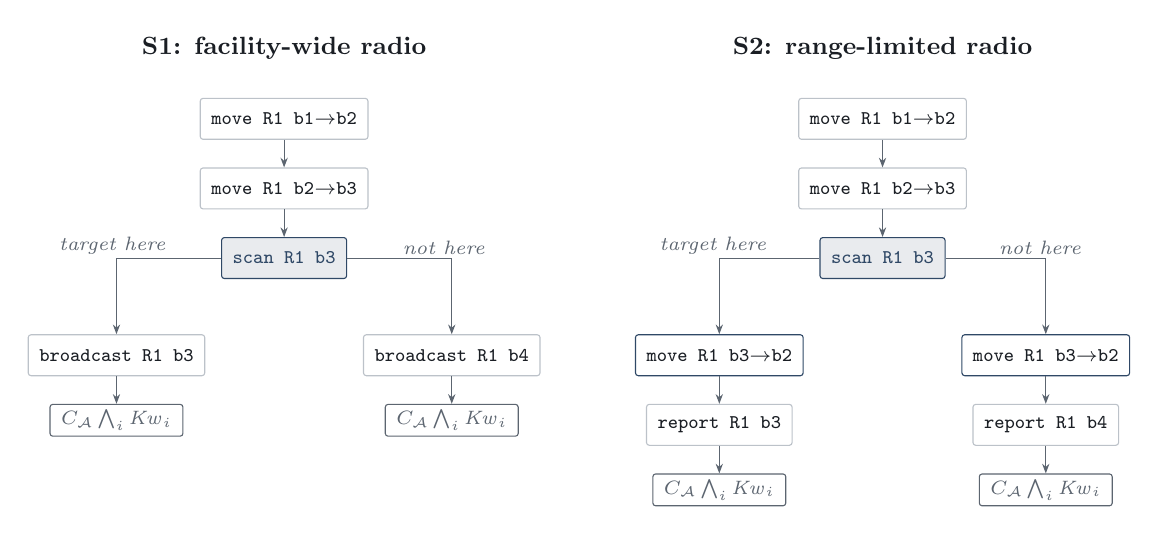
\begin{tikzpicture}[
    act/.style={draw=rulegrey, fill=white, rounded corners=1pt, font=\scriptsize\ttfamily,
                text=ink, inner xsep=4pt, inner ysep=2.5pt, minimum height=5.2mm},
    sens/.style={act, draw=steel, fill=mist, text=steel, font=\scriptsize\ttfamily\bfseries},
    goalnode/.style={draw=slate, fill=white, font=\scriptsize\itshape, text=slate,
                     rounded corners=1pt, inner xsep=4pt, inner ysep=2pt},
    ed/.style={-{Stealth[length=3.5pt]}, draw=slate},
    brl/.style={font=\scriptsize\itshape, text=slate, inner sep=1pt},
    hdr/.style={font=\small\bfseries, text=ink}
  ]
  % ---------------- public ----------------
  \node[hdr] (h1) at (0,0.9) {S1: facility-wide radio};
  \node[act] (p1) at (0,0) {move R1 b1$\to$b2};
  \node[act, below=3.5mm of p1] (p2) {move R1 b2$\to$b3};
  \node[sens, below=3.5mm of p2] (p3) {scan R1 b3};
  \node[act, below left=7mm and 2mm of p3] (p4a) {broadcast R1 b3};
  \node[act, below right=7mm and 2mm of p3] (p4b) {broadcast R1 b4};
  \node[goalnode, below=3.5mm of p4a] (g1a) {$\Cop{\Ag}\bigwedge_i \Kw{i}$};
  \node[goalnode, below=3.5mm of p4b] (g1b) {$\Cop{\Ag}\bigwedge_i \Kw{i}$};
  \draw[ed] (p1) -- (p2); \draw[ed] (p2) -- (p3);
  \draw[ed] (p3) -| (p4a) node[brl, pos=0.25, above left] {target here};
  \draw[ed] (p3) -| (p4b) node[brl, pos=0.25, above right] {not here};
  \draw[ed] (p4a) -- (g1a); \draw[ed] (p4b) -- (g1b);

  % ---------------- radio ----------------
  \begin{scope}[xshift=7.6cm]
  \node[hdr] (h2) at (0,0.9) {S2: range-limited radio};
  \node[act] (q1) at (0,0) {move R1 b1$\to$b2};
  \node[act, below=3.5mm of q1] (q2) {move R1 b2$\to$b3};
  \node[sens, below=3.5mm of q2] (q3) {scan R1 b3};
  \node[act, below left=7mm and 2mm of q3, draw=steel] (q4a) {move R1 b3$\to$b2};
  \node[act, below right=7mm and 2mm of q3, draw=steel] (q4b) {move R1 b3$\to$b2};
  \node[act, below=3.5mm of q4a] (q5a) {report R1 b3};
  \node[act, below=3.5mm of q4b] (q5b) {report R1 b4};
  \node[goalnode, below=3.5mm of q5a] (g2a) {$\Cop{\Ag}\bigwedge_i \Kw{i}$};
  \node[goalnode, below=3.5mm of q5b] (g2b) {$\Cop{\Ag}\bigwedge_i \Kw{i}$};
  \draw[ed] (q1) -- (q2); \draw[ed] (q2) -- (q3);
  \draw[ed] (q3) -| (q4a) node[brl, pos=0.25, above left] {target here};
  \draw[ed] (q3) -| (q4b) node[brl, pos=0.25, above right] {not here};
  \draw[ed] (q4a) -- (q5a); \draw[ed] (q4b) -- (q5b);
  \draw[ed] (q5a) -- (g2a); \draw[ed] (q5b) -- (g2b);
  \end{scope}
\end{tikzpicture}
\caption{Policies synthesised for the same instance shape under the two
communication models (3 UGVs, 4 bays, target in $\{b_3,b_4\}$, depot start,
common-knowledge goal). Branches are the designated events of the sensing
action. Two behaviours are worth noting: on the negative branch the planner
reports \texttt{b4}, a bay no vehicle ever scanned, because the reading plus
the common knowledge that the target is in exactly one of the two bays entails
it; and under the range-limited radio it inserts a return move on \emph{both}
branches, since the report is worthless outside the depot's radio
neighbourhood.}
\label{fig:policies}
\end{figure}

The interaction view of the same range-limited policy
(Figure~\ref{fig:interaction}) makes the obliviousness explicit: during the
excursion to $b_3$ the other two vehicles observe nothing at all, not the
movement's informational content, not the scan, not that a reading was
obtained, and the fleet's knowledge state changes only at the moment the
report is transmitted from within range.

\begin{figure}[H]
\centering
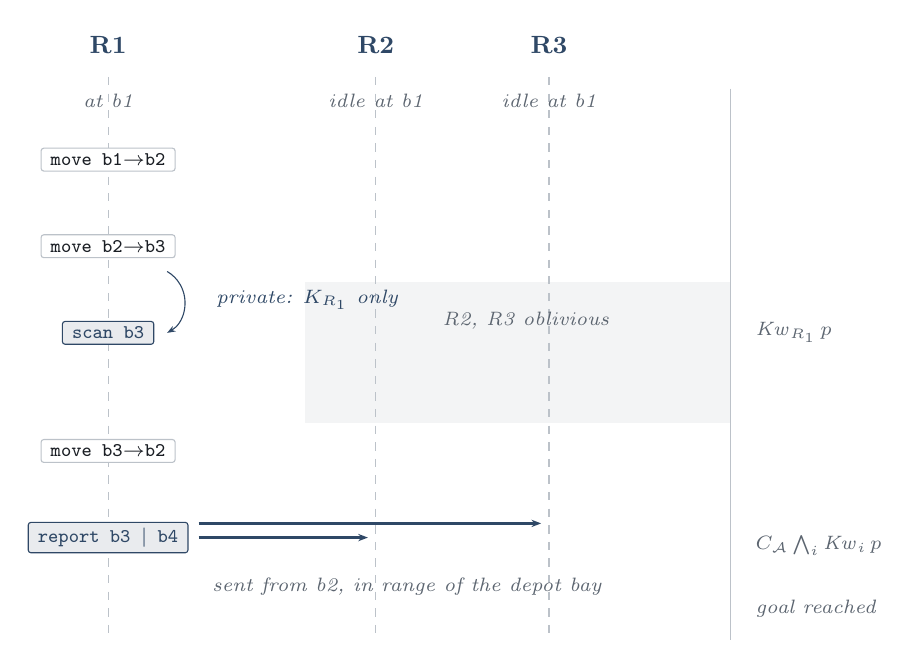
\begin{tikzpicture}[
    lane/.style={draw=rulegrey, dashed},
    lbl/.style={font=\small\bfseries, text=steel},
    ev/.style={draw=rulegrey, fill=white, font=\scriptsize\ttfamily, text=ink,
               inner xsep=3.5pt, inner ysep=2pt, rounded corners=1pt},
    evs/.style={ev, draw=steel, fill=mist, text=steel},
    msg/.style={-{Stealth[length=3.5pt]}, draw=steel, thick},
    note/.style={font=\scriptsize\itshape, text=slate, anchor=west}
  ]
  \def\ta{-0.9} \def\tb{-2.0} \def\tc{-3.1} \def\td{-4.6} \def\te{-5.7}
  % lanes
  \foreach \x/\n in {0/R1, 3.4/R2, 5.6/R3} {
      \node[lbl] at (\x,0.55) {\n};
      \draw[lane] (\x,0.15) -- (\x,-7.0);
  }
  \node[font=\scriptsize\itshape, text=slate] at (0,-0.15) {at b1};
  \node[font=\scriptsize\itshape, text=slate] at (3.4,-0.15) {idle at b1};
  \node[font=\scriptsize\itshape, text=slate] at (5.6,-0.15) {idle at b1};
  % oblivious band
  \begin{scope}[on background layer]
    \fill[slate, opacity=0.07] (2.5,\tb-0.45) rectangle (7.9,\td+0.35);
  \end{scope}
  \node[note, text=slate] at (6.05,-3.6) {};
  \node[font=\scriptsize\itshape, text=slate] at (5.2,\tc+0.15)
       {\ \ R2, R3 oblivious};

  % events on R1
  \node[ev] at (0,\ta) {move b1$\to$b2};
  \node[ev] at (0,\tb) {move b2$\to$b3};
  \node[evs] at (0,\tc) {scan b3};
  \node[ev] at (0,\td) {move b3$\to$b2};
  \node[evs] at (0,\te) {report b3 $|$ b4};

  % private sensing self-loop
  \draw[{Stealth[length=3pt]}-, draw=steel]
       (0.75,\tc) arc (-60:60:0.45) ;
  \node[note, text=steel] at (1.25,\tc+0.42) {private: $\Kop{R_1}$ only};

  % report reaches both, in range
  \draw[msg] (1.15,\te) -- (3.3,\te);
  \draw[msg] (1.15,\te+0.18) -- (5.5,\te+0.18);
  \node[note] at (1.2,\te-0.62) {sent from b2, in range of the depot bay};

  % knowledge annotations
  \draw[draw=rulegrey] (7.9,0) -- (7.9,-7.0);
  \node[note] at (8.1,\tc) {$\Kw{R_1}\,p$};
  \node[note] at (8.1,\te-0.1) {$\Cop{\Ag}\bigwedge_i \Kw{i}\,p$};
  \node[note, text=slate] at (8.1,-6.6) {goal reached};
\end{tikzpicture}
\caption{Interaction view of the range-limited policy of
Figure~\ref{fig:policies}, with $p \equiv \mathit{target\text{-}at}(b_3)$. The
shaded interval is the excursion during which R2 and R3 are oblivious: they do
not observe the scan, and therefore cannot infer from R1's silence that a
reading was taken. Fleet knowledge changes only at the transmission.}
\label{fig:interaction}
\end{figure}

The facility family produces the one policy shape the corridor families cannot:
a capability interlock, in which one vehicle changes the world so that another
can learn something. Figure~\ref{fig:interlock} is the solver's output on
\texttt{facility-a2-b4-i1-depot-ck}.

\begin{figure}[H]
\centering
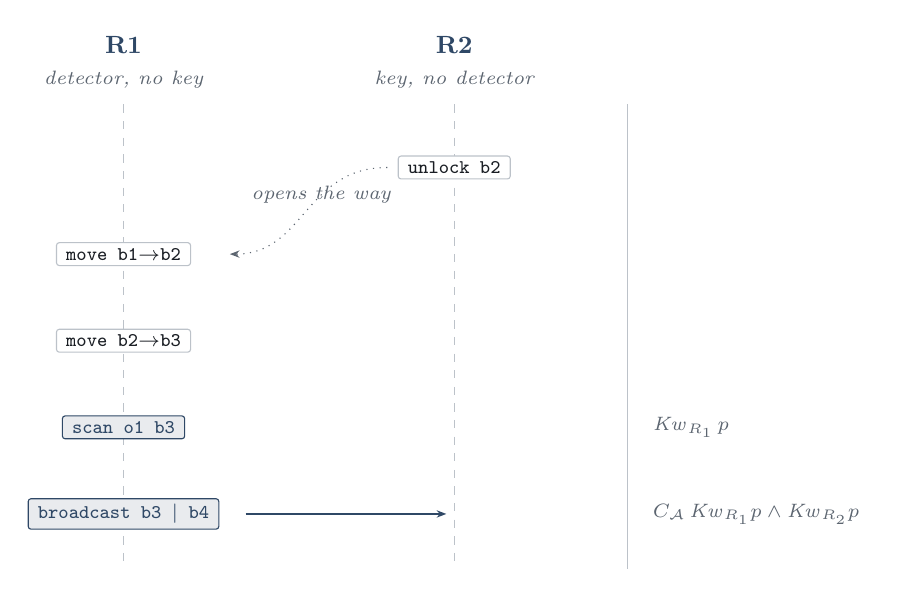
\begin{tikzpicture}[
    lane/.style={draw=rulegrey, dashed},
    lbl/.style={font=\small\bfseries, text=steel},
    role/.style={font=\scriptsize\itshape, text=slate},
    ev/.style={draw=rulegrey, fill=white, font=\scriptsize\ttfamily, text=ink,
               inner xsep=3.5pt, inner ysep=2pt, rounded corners=1pt},
    evs/.style={ev, draw=steel, fill=mist, text=steel},
    dep/.style={-{Stealth[length=3.5pt]}, draw=slate, dotted},
    msg/.style={-{Stealth[length=3.5pt]}, draw=steel, thick},
    note/.style={font=\scriptsize\itshape, text=slate, anchor=west}
  ]
  \def\ta{-1.0} \def\tb{-2.1} \def\tc{-3.2} \def\td{-4.3} \def\te{-5.4}
  \node[lbl] at (0,0.55) {R1}; \node[role] at (0,0.12) {detector, no key};
  \node[lbl] at (4.2,0.55) {R2}; \node[role] at (4.2,0.12) {key, no detector};
  \draw[lane] (0,-0.2) -- (0,-6.1);
  \draw[lane] (4.2,-0.2) -- (4.2,-6.1);

  \node[ev] at (4.2,\ta) {unlock b2};
  \node[ev] at (0,\tb) {move b1$\to$b2};
  \node[ev] at (0,\tc) {move b2$\to$b3};
  \node[evs] at (0,\td) {scan o1 b3};
  \node[evs] at (0,\te) {broadcast b3 $|$ b4};

  \draw[dep] (3.35,\ta) .. controls (2.3,\ta) and (2.3,\tb) .. (1.35,\tb);
  \node[note] at (1.5,\ta-0.34) {opens the way};

  \draw[msg] (1.55,\te) -- (4.1,\te);

  \draw[draw=rulegrey] (6.4,-0.2) -- (6.4,-6.1);
  \node[note] at (6.6,\td) {$\Kw{R_1}\,p$};
  \node[note] at (6.6,\te) {$\Cop{\Ag}\,\Kw{R_1}p \wedge \Kw{R_2}p$};
\end{tikzpicture}
\caption{Capability interlock on \texttt{facility-a2-b4-i1-depot-ck}. R2 holds
the key but no detector and R1 the reverse, so the ontic action of one vehicle
is the precondition for the epistemic action of the other. The final broadcast
is what turns R1's private reading into the fleet-wide common knowledge the
goal demands.}
\label{fig:interlock}
\end{figure}

\subsection{A correctness discrepancy}
\label{sec:discrepancy}

Four of the 204 policies do not withstand inspection, and the benchmark is
reported here partly because it found them. In each of the four multi-item
facility instances, the policy ends on a \emph{private} scan with no
subsequent broadcast, while the goal requires common knowledge across the
fleet. On \texttt{facility-a2-b5-i2-depot-ck} the tail is

\begin{lstlisting}[caption={The suspect tail: R1 senses privately and the
policy terminates, although the goal demands that R2 know as well.}]
    ... broadcast_R1_o2_b2 -> unlock_R2_b2_b3
        -> move_R1_b2_b3 -> move_R1_b3_b4 -> scan_R1_o1_b4  [leaf]
\end{lstlisting}

Since \texttt{scan} declares \texttt{(default Oblivious)}, R2 does not observe
the reading, nor that a scan occurred; its accessibility class after the update
still contains worlds disagreeing on the item's bay, so $\Kw{R_2}$ fails and
the goal cannot hold at that leaf. Three independent checks agree. First,
\textsf{plank}'s own validator, run on the same history, reports the goal
unsatisfied. Second, the identical instance with a goal naming only the
last-scanned item is solved correctly, with the broadcast present, so the
model and the domain are not at fault. Third, the same instance shape with a
single item, and every one of the 190 corridor and addressed-radio policies,
ends in a communication action as it should; only goals that conjoin
knowledge requirements over \emph{two distinct atoms} exhibit the fault.

The defect therefore sits in the planner rather than in the encoding, and its
signature is narrow: a conjunctive goal over several atoms is accepted in a
state where only the most recently sensed conjunct holds for the sensing agent.
The formula evaluator and the goal test itself read correctly, which points at
the branch states the AO$^\ast$ layer evaluates, the split-and-contract step
,  rather than at satisfaction checking. The four affected instances are
excluded from no aggregate in this report, because their \emph{cost} figures
remain valid measurements of the search that was performed; but their
\emph{solved} status should be read as unconfirmed, and the extended coverage
figure of 60/60 as 56/60 confirmed.

\subsection{Scaling}

\begin{figure}[H]
\centering
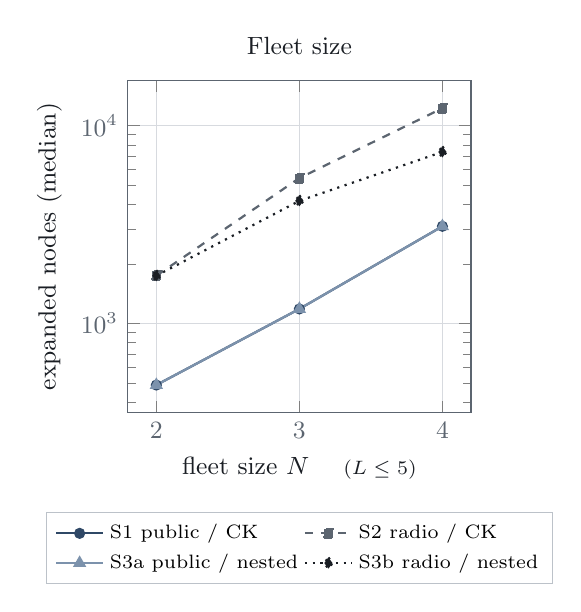
\begin{tikzpicture}
\begin{axis}[
    width=0.49\textwidth, height=5.8cm,
    ymode=log, log basis y=10,
    ylabel={expanded nodes (median)},
    grid=major, grid style={draw=rulegrey!60, very thin},
    axis line style={draw=slate}, tick label style={font=\small, color=slate},
    label style={font=\small, color=ink}, title style={font=\small, color=ink},
    legend style={font=\scriptsize, draw=rulegrey, fill=white, at={(0.5,-0.30)},
                  anchor=north, legend columns=2, cells={anchor=west}},
    cycle list={
        {steel, mark=*, mark size=1.6pt, thick},
        {slate, mark=square*, mark size=1.6pt, thick, dashed},
        {steellight, mark=triangle*, mark size=2pt, thick},
        {ink, mark=diamond*, mark size=2pt, thick, dotted}},
    xlabel={fleet size $N$ \quad{\scriptsize($L\le5$)}}, title={Fleet size}, xtick={2,3,4},
]
\addplot coordinates {(2,487) (3,1182) (4,3096)};
\addlegendentry{S1 public / CK}
\addplot coordinates {(2,1740) (3,5430) (4,12251)};
\addlegendentry{S2 radio / CK}
\addplot coordinates {(2,487) (3,1182) (4,3096)};
\addlegendentry{S3a public / nested}
\addplot coordinates {(2,1740) (3,4164) (4,7365)};
\addlegendentry{S3b radio / nested}
\end{axis}
\end{tikzpicture}
\hfill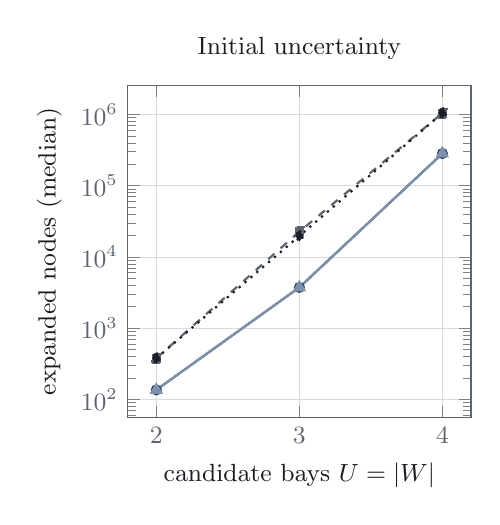
\begin{tikzpicture}
\begin{axis}[
    width=0.49\textwidth, height=5.8cm,
    ymode=log, log basis y=10,
    ylabel={expanded nodes (median)},
    grid=major, grid style={draw=rulegrey!60, very thin},
    axis line style={draw=slate}, tick label style={font=\small, color=slate},
    label style={font=\small, color=ink}, title style={font=\small, color=ink},
    legend style={font=\scriptsize, draw=rulegrey, fill=white, at={(0.5,-0.30)},
                  anchor=north, legend columns=2, cells={anchor=west}},
    cycle list={
        {steel, mark=*, mark size=1.6pt, thick},
        {slate, mark=square*, mark size=1.6pt, thick, dashed},
        {steellight, mark=triangle*, mark size=2pt, thick},
        {ink, mark=diamond*, mark size=2pt, thick, dotted}},
    xlabel={candidate bays $U = |W|$}, title={Initial uncertainty}, xtick={2,3,4},
    legend style={draw=none, fill=none},
]
\addplot coordinates {(2,136) (3,3736) (4,283160)};
\addplot coordinates {(2,378) (3,22644) (4,1045482)};
\addplot coordinates {(2,136) (3,3736) (4,283160)};
\addplot coordinates {(2,378) (3,19678) (4,1045482)};
\end{axis}
\end{tikzpicture}

\caption{Search effort against the two parameters that matter, on logarithmic
axes; each point is a median over solved instances. Left: fleet size,
restricted to $L\le5$ because the $L=6$ stratum of the grid always carries
$U=4$ and would otherwise confound the two. Right: initial uncertainty, which
is also the world count $|W|$ of the initial model; note the wider vertical
range, uncertainty moves the cost by three orders of magnitude, fleet size
by about one. The two public series coincide throughout: under a facility-wide
radio a nested goal is reached by the same policy as the common-knowledge one.
Legend shared by both panels.}
\label{fig:scaling}
\end{figure}

\subsection{Reading of the measurements}

\paragraph{Initial uncertainty is the dominant cost}
Holding the fleet at $N=2$, the median expanded-node count rises from 172
($U=2$) to 2\,177 ($U=3$) to 330\,188 ($U=4$). Since every candidate bay
contributes one world to the initial model, $U$ \emph{is} $|W|$, and each extra
world multiplies both the size of every model along the frontier and the number
of branches a policy must cover. Nothing else in the grid moves the cost by
three orders of magnitude.

\paragraph{Fleet size is secondary, corridor length intermediate}
Restricted to $L\le5$ so the uncertainty frontier does not confound it, fleet
size takes the median from 621 ($N=2$) to 2\,714 ($N=3$) to 5\,480 ($N=4$) , 
roughly an order of magnitude across the range, not three. Corridor length at
fixed $U=2$ gives 66, 214, 2\,801 for $L=3,4,5$: longer corridors buy longer
plans, and depth costs more than breadth here.

\paragraph{Restricted communication costs about a factor of three}
At matched corridor length, the range-limited domain expands roughly $3\times$
the nodes of the public one ($L=4$: 2\,184 vs.\ 734; $L=5$: 28\,000 vs.\
2\,177) and produces policies one to three steps deeper. The extra depth is the
return-into-range or relay move, and it appears on \emph{every} branch, so it
multiplies rather than adds. All eight unsolved instances are range-limited.

\paragraph{Second-order goals were not the bottleneck}
Nested goals cost no more than common-knowledge goals in this grid (median
2\,224 vs.\ 2\,532 expanded). Under a public radio this is expected, one
announcement gives common knowledge, which entails any finite nesting. Under
the range-limited radio the nested goal is \emph{weaker} than the
common-knowledge one: it constrains two vehicles rather than the whole fleet,
so it is reached by a prefix of the same policy. A genuinely harder
second-order task would require the sender to establish receipt without the
receiver's position being common knowledge, which this instance family does not
construct.

\paragraph{Grounding and search fail in opposite directions}
Search cost tracks $U$; grounding cost tracks $N\times L$. Ground actions grow
from 20 to 88 across the grid, and \textsf{plank}'s grounding time from 0.02\,s
to 76\,s, the worst case being $N=4$, $L=6$, an instance whose \emph{search},
where solved, takes a few seconds. For a fielded system these are different
engineering problems: grounding is an offline, cacheable cost that scales with
the size of the facility and the fleet, while search is the online cost and
scales with how much the fleet does not know.

\paragraph{The selection policy did not discriminate}
The planner's automatic policy chose \texttt{knowledge-spread} with AO$^\ast$
for all 136 solved instances (Table~\ref{tab:selection}). This is a reasonable
classification, every instance has sensing, a knowing-whether goal, and few
designated worlds, but it means the benchmark exercises one configuration
and says nothing about the alternatives. Instances that would discriminate
between heuristics need goals mixing modal and factual conjuncts, which this
family deliberately avoids.


%======================================================================
\section{Discussion}

\paragraph{What the numbers say about the formulation}
The measurements separate two costs that are easy to conflate, and they fail in
opposite directions. Grounding cost is combinatorial in the
\emph{specification}: ground actions grow as $O(N\cdot L)$, and grounding time
followed, from 0.02\,s to 76\,s across the grid. Search cost is combinatorial
in the \emph{model}: each product update multiplies the world count by the
number of applicable designated events, so the initial world count, here
exactly the number of candidate bays, compounds at every step, which is why
it moved the median expanded count by three orders of magnitude while fleet
size moved it by one. The practical consequence is that the two scale along
different axes of a deployment: a bigger facility with a bigger fleet is a
grounding problem, and can be paid for offline; a fleet that knows less is a
search problem, and must be paid for online.

\paragraph{Where the epistemic formulation pays}
The negative-scan inference of S1 and the delivery reasoning of S2 and S3 are
not accessible to a classical encoding without hand-written epistemic
bookkeeping: one would have to introduce propositions such as
\texttt{knows-R1-target-at-b4} and axiomatise their dynamics by hand, per
domain, and re-do that work whenever the observability model changes. In the
DEL encoding, changing the radio from facility-wide to range-limited is a
change to one observability condition, and every consequence, including that
an out-of-range vehicle cannot infer anything from silence, follows from the
product update rather than from the modeller's diligence.

\paragraph{Where it does not}
Coverage is high, 136 of 144, most in milliseconds, but the grid is
small, and the wall is close: four candidate bays under a range-limited radio
already defeats a 60\,s budget for fleets of three and four. This is a property
of explicit-state DEL planning, not of the encoding: the representation is a
Kripke model that is copied and grown at every step. Work on symbolic and
factored epistemic state representations, and on planners that restrict to a
bounded modal depth, targets exactly this. For a fielded fleet, the realistic
reading is that DEL is the right language for the \emph{coordination layer} , 
a handful of vehicles deciding who scans and who speaks, over a coarse
partition of the map and a small number of open hypotheses, and not for the
metric layer beneath it.

\paragraph{What a benchmark is for}
Section~\ref{sec:discrepancy} is the part of this study that would not have
been obtained by reasoning about the formalism. A suite that only varies size
exercises one code path more heavily; a suite that varies the \emph{shape} of
the goal, knowing-whether against nested against negated against conjoined
over several atoms, exercises different ones, and the fault surfaced only on
the last of those. The practical lesson for building epistemic domains is to
treat goal shape as a benchmark dimension of the same standing as fleet size,
and to keep an independent checker in the loop: here \textsf{plank}'s validator
adjudicated a disagreement that the planner's own validator could not, since it
shares the state pipeline under suspicion.

\paragraph{Threats to the reading}
Four caveats. The corridor topology is a path, the easiest possible
adjacency structure; a branching facility graph would raise the movement
branching factor without changing the epistemic content, and the separation
between the two costs reported above would be less clean. The measurements come
from a single planner configuration chosen automatically per instance, so they
characterise that policy and not the intrinsic difficulty of the tasks. And
the 60~s limit is short by planning-competition standards; unsolved instances
should be read as \emph{not solved under this budget}, not as unsolvable.
Finally, four returned policies are known to be wrong
(Section~\ref{sec:discrepancy}), and the remainder were checked only by the
planner's own validator, so other faults of the same kind would not have been
detected.

%======================================================================
\section{Conclusion}

The coordination problem for a UGV fleet with local sensing and limited
communication is naturally a problem about knowledge, and DEL states it
directly: epistemic states as Kripke models, actions as event models whose
observability relations decide who learns what, plans as policies branching on
sensing outcomes, and goals as modal formulas including common knowledge and
nested knowledge. The four scenario families in Section~\ref{sec:scenarios}
show that the interesting variation, inference from a negative reading,
delivery past obliviousness, confirmation of receipt, lives entirely in the
observability model, and that changing it is a local change to the
specification rather than a re-derivation of the domain.

The benchmark quantifies the price. The binding constraint is not the size of
the fleet or of the facility but the number of hypotheses the fleet starts
with: uncertainty enters the model multiplicatively and dominates everything
else by two orders of magnitude, while fleet size and facility size are largely
a grounding cost that can be paid offline. Restricted communication adds a
constant factor and, in this grid, all of the failures.

That profile is the useful design guidance. Keep the epistemic layer's
hypothesis space small, let the perception and mapping layers prune
candidates before the task layer ever sees them, and spend the modelling
budget on the communication structure, which is both where the interesting
coordination lives and where a change costs a single observability condition.

%======================================================================
\appendix
\section{Reproduction}

\begin{lstlisting}[language=bash, morekeywords={python3,cd}, caption={Regenerating the benchmark from scratch.}]
cd epddl-workspace/ugv-coordination
python3 gen_instances.py             ; 144 corridor instances  -> instances/
python3 gen_instances_x.py           ;  60 extended instances  -> instances/
python3 run_benchmark.py             ; grounds + solves all, writes results.csv
python3 run_benchmark.py directed    ; or re-run one family, merging results
python3 make_tables.py               ; regenerates the tables in this report
\end{lstlisting}

A single instance can be traced end to end with:

\begin{lstlisting}[language=bash, caption={Grounding and solving one instance.}]
plank export -d domains/ugv-radio.epddl \
             -p instances/radio-a3-b4-u2-depot-nested.epddl \
             -l ~/plank/benchmarks/libraries/intermediate.epddl -o export_out

epistemic_planner --task export_out/radio-a3-b4-u2-depot-nested.json \
                  --plan plans/radio-a3-b4-u2-depot-nested.json --explain
\end{lstlisting}

\begin{thebibliography}{9}
\small
\bibitem{ditmarsch2007}
H.~van Ditmarsch, W.~van der Hoek, and B.~Kooi.
\emph{Dynamic Epistemic Logic}. Springer, 2007.

\bibitem{baltag1998}
A.~Baltag, L.~S. Moss, and S.~Solecki.
The logic of public announcements, common knowledge, and private suspicions.
\emph{Proc. TARK}, 1998.

\bibitem{fagin1995}
R.~Fagin, J.~Y. Halpern, Y.~Moses, and M.~Y. Vardi.
\emph{Reasoning About Knowledge}. MIT Press, 1995.

\bibitem{bolander2011}
T.~Bolander and M.~B. Andersen.
Epistemic planning for single- and multi-agent systems.
\emph{Journal of Applied Non-Classical Logics}, 21(1):9--34, 2011.

\bibitem{muise2015}
C.~Muise et al.
Planning over multi-agent epistemic states: a classical planning approach.
\emph{Proc. AAAI}, 2015.

\bibitem{kominis2015}
F.~Kominis and H.~Geffner.
Beliefs in multiagent planning: from one agent to many.
\emph{Proc. ICAPS}, 2015.

\bibitem{fabiano2020}
F.~Fabiano, A.~Burigana, A.~Dovier, and E.~Pontelli.
EFP 2.0: a multi-agent epistemic solver with multiple e-state representations.
\emph{Proc. ICAPS}, 2020.

\bibitem{plank}
A.~Burigana. \textsf{plank}: a DEL-based epistemic planning toolkit.
Software, \url{https://github.com/a-burigana/plank}.

\bibitem{aletheia}
\textsf{aletheia}: an explicit-state DEL epistemic planner. Software.
\end{thebibliography}

\end{document}
